\documentclass[tikz]{standalone}
\usetikzlibrary{positioning}

\newcommand{\po}{\texttt{po}}
\renewcommand{\wr}{\texttt{wr}}
\newcommand{\rd}{\texttt{rd}}

\newcommand{\povis}[2]{\draw [->, thick] (#1) to node[above] {\Large{\po}} (#2);}
\newcommand{\vis}[2]{\draw [->, thick] (#1) to node[above, sloped, pos=0.7] {\Large{\texttt{rf}}} (#2);}
\newcommand{\porf}[2]{\draw [->, thick] (#1) to [out=345,in=195] node[above, pos = 0.6] {\Large{\texttt{rf}}} (#2);}
%\newcommand{\porf}[2]{\draw [->, thick] (#1) to [out=20,in=160] node[above, pos = 0.8] {\Large{\texttt{rf}}} (#2);}

\begin{document}
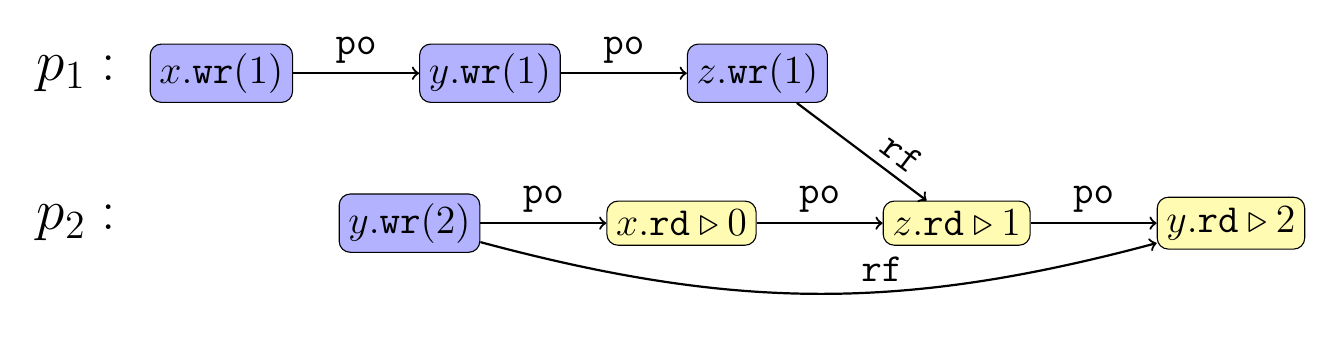
\begin{tikzpicture}
\tikzset{
  wop/.style = {rectangle, rounded corners, fill = blue!30, draw, font = \Large},
  rop/.style = {rectangle, rounded corners, fill = yellow!30, draw, font = \Large}, process/.style = {font = \huge},
  %po/.style = {->, very thick},
  rw/.style = {->, shorten >= 3pt, very thick, dashed},
  %vis/.style = {->, shorten >= 3pt, very thick, dashed}
}

  \node (p1) [process] {$p_1:$};
  \node (wx1) [wop, right = 0.3cm of p1] {$x.\wr(1)$};
  \node (wy1) [wop, right = 1.6cm of wx1] {$y.\wr(1)$};
  \node (wz1) [wop, right = 1.6cm of wy1] {$z.\wr(1)$};

  \node (p2) [process, below = 1.2cm of p1] {$p_2:$};
  \node (wy2) [wop, right = 2.7cm of p2] {$y.\wr(2)$};
  \node (rx0) [rop, right = 1.6cm of wy2] {$x.\rd\triangleright0$};
  \node (rz1) [rop, right = 1.6cm of rx0] {$z.\rd\triangleright1$};
  \node (ry2) [rop, right = 1.6cm of rz1] {$y.\rd\triangleright2$};

  \povis{wx1}{wy1};
  \povis{wy1}{wz1};

  \povis{wy2}{rx0};
  \povis{rx0}{rz1};
  \povis{rz1}{ry2};

  \vis{wz1}{rz1};
  \porf{wy2}{ry2};

\end{tikzpicture}
\end{document}
